\chapter{Metodologia}\label{chp:metodologia}
\section{Modelagem matemática}
\subsection{Adesivo transdérmico}

A modelagem matemática do adesivo transdérmico foi realizada utilizando a Segunda Lei de Fick para descrever a difusão do EE através da camada adesiva, seguindo o modelo de Simon (2007). Dado que o objetivo principal deste trabalho é analisar a difusão do etinilestradiol nas matrizes, e sendo a matriz adesiva a responsável pela liberação controlada do fármaco, tomou-se a decisão de concentrar a análise nessa camada. A difusão do EE através da camada adesiva foi considerada significativamente mais lenta do que a absorção na pele e nos vasos sanguíneos, representando a etapa limitante do processo. Dessa forma, optou-se por desconsiderar a camada da pele, simplificando o modelo sem perda de representatividade para o caso limite do estudo. Assim, foi considerada apenas a EDP correspondente à camada adesiva:

\begin{equation}
\frac{\partial C_1}{\partial t} = D_1 \frac{\partial^2 C_1}{\partial x^2}, \quad 0 < x < L_1, \quad 0 < t \leq T
\end{equation}

\noindent sendo $C_1$ a concentração de etinilestradiol e $D_1$ o coeficiente de difusão na camada adesiva, $L_1$ a espessura da camada e $T$ o período de aplicação.

A fim de calcular a concentração inicial, foi primeiro calculado o volume ocupado pela camada adesiva. Para isso, foi utilizado o valor de 0,004 cm para a espessura do adesivo (Simon, 2007) e a área superficial de 20 cm\textsuperscript{2} (Devineni, 2007).

\begin{equation}
    V = A \cdot L_1 
\end{equation}
\begin{equation}
    V = 20 \cdot 0,004 = 0,08 cm\textsuperscript{3}
\end{equation}

A dosagem considerada foi de 750 \textmu g de etinilestradiol por adesivo (Devineni, 2007) e supõe-se que a concentração seja uniforme ao longo da matriz. Dessa forma, a concentração inicial pode ser obtida por: 

\begin{equation}
C_1[x,0] = C_{10}, \quad 0 < x < L_1
\end{equation}
\begin{equation}
    C_{10} = \frac{750 \, \mu g}{0,08 \, cm\textsuperscript{3}} =  9375 \, \mu g/cm\textsuperscript{3}
\end{equation}

Para o coeficiente de difusão, foi considerado o trabalho de Rohr e Saeger‐Lorenz (2002), no qual foi estudado o coeficiente de difusão do $17\beta$-estradiol em uma matriz adesiva. Devido à ausência de dados na literatura sobre o coeficiente de difusão do etinilestradiol nesse tipo de matriz, foi necessário realizar uma aproximação a partir desse valor. Sabe-se que o coeficiente de difusão é influenciado por vários fatores, entre eles o tamanho, a forma e a flexibilidade da molécula em difusão. Sabe-se também que seu valor é inversamente proporcional ao raio da molécula (Kreilgaard et. al, 2000). Assim, devido à adição do grupo etinil causar aumento do raio da molécula, considera-se esse valor como uma aproximação inicial, sendo que o coeficiente de difusão real do etinilestradiol será um valor menor a ser determinado empiricamente durante a modelagem computacional. Convertendo o valor obtido na literatura para cm\textsuperscript{2}/h, tem-se:

\begin{equation}
    D_1 = 7,2 \times 10^{-11} \, cm\textsuperscript{2}/s \times 3600 \, \text{s/h} = 2,59 \times 10^{-7} \, cm\textsuperscript{2}/h
\end{equation}

Para as condições de contorno, foi considerado que na borda exterior, $x = 0$, o fluxo é nulo, devido ao sistema possuir uma quantidade finita de fármaco. Na borda mais próxima da pele, $x = L$, foi definida uma condição de partição utilizando coeficiente $Km = 1$ (Simon, 2007), indicando que a concentração do fármaco é a mesma na matriz e na pele em equilíbrio. Essas condições podem ser visualizadas na Eq. (3.7) e Eq. (3.8) abaixo.

\begin{equation}
\frac{\partial C_1(0,t)}{\partial x} = 0, \quad 0 < t \leq T
\end{equation}

\begin{equation}
K_m C_1(L_1,t) = C_{pele}, \quad 0 < t \leq T
\end{equation}

A \Tabela{tab:tabela_1} contém um resumo dos parâmetros utilizados nesse modelo.

\begin{table}[!htp]
\caption[Parâmetros para o adesivo transdérmico]{Parâmetros utilizados para o modelo do adesivo transdérmico}
\label{tab:tabela_1}
\begin{center}
\begin{tabular}{ccc}
\toprule % Linha superior
Parâmetro & Valor & Referência \\ \midrule % Linha do meio 
\textbf{$D_1$}  & $5,184 \times 10^{-8} \, cm\textsuperscript{2}/h$ & Rohr e Saeger-Lorenz (2002) \\
\textbf{$C_{10}$} & 9375 \textmu g/cm\textsuperscript{3} & Devineni (2007) \\
\textbf{$L_1$}  & 0,004 cm & Simon (2007) \\
\textbf{$K_m$} & 1 & Simon (2007) \\\bottomrule % Linha inferior
\end{tabular}
\end{center}
\end{table}

\subsection{Anel vaginal}

A modelagem matemática do anel vaginal foi realizada de maneira análoga à da camada adesiva, sendo sua EDP correspondente:

\begin{equation}
\frac{\partial C_2}{\partial t} = D_2 \frac{\partial^2 C_2}{\partial x^2}, \quad 0 < x < L_2, \quad 0 < t \leq T
\end{equation}

A fim de calcular a concentração inicial, foi necessário primeiro calcular o volume do anel. O anel vaginal pode ser definido como um toróide oco, conforme mostra a \Figura{fig:anel_vaginal} abaixo:

\begin{figure}[!htb]
    \centering
        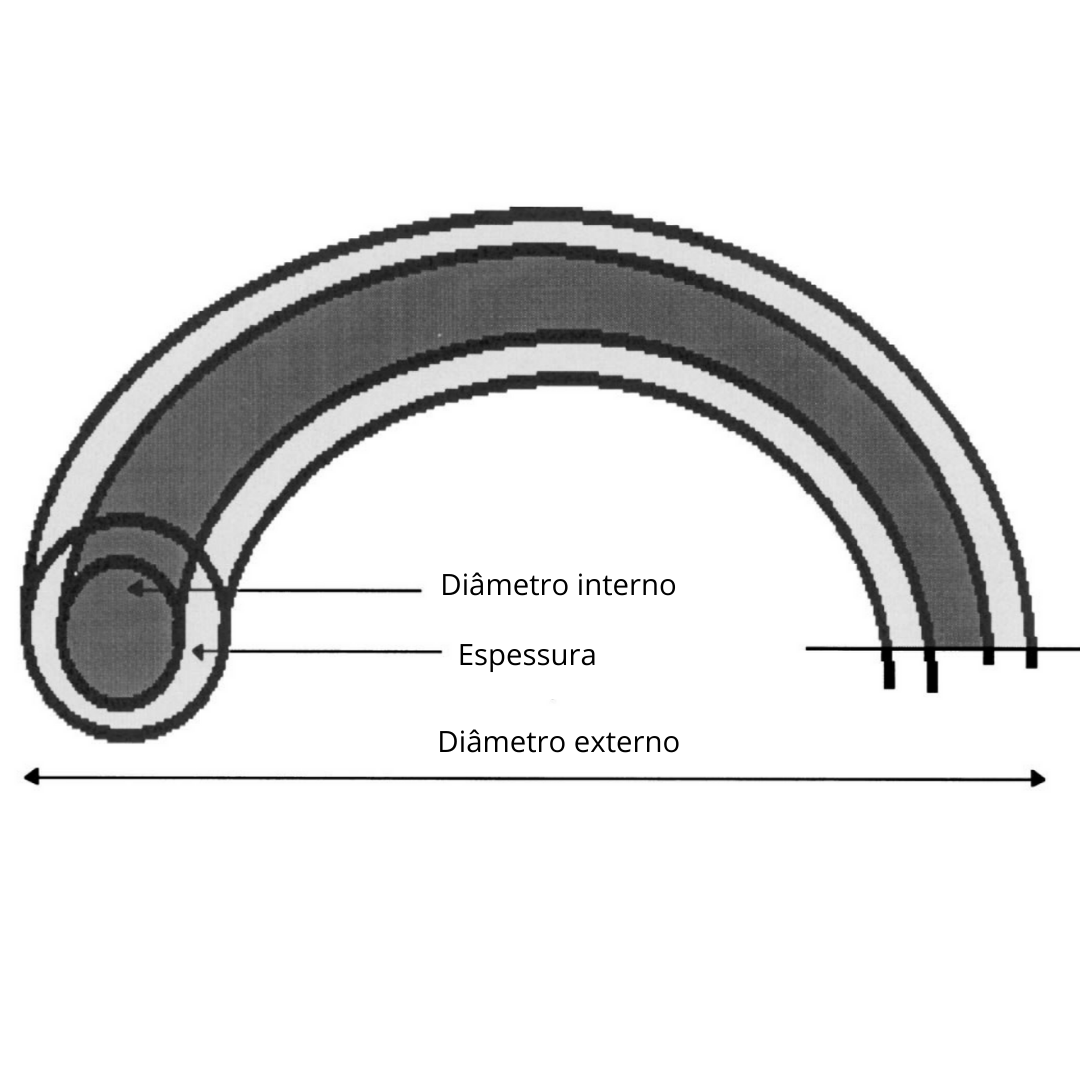
\includegraphics[width=0.48\textwidth]{figuras/anel_vaginal.png}
        \caption[Geometria de um anel vaginal]{Geometria de um anel vaginal (Woolfson et. al, 1999).}
    \label{fig:anel_vaginal}
\end{figure}

Assim, é necessário calcular o volume do toróide externo e subtrair o volume do toróide interno. De Barnhart et. al (2005), de acordo com as especificações do NuvaRing{\textregistered}, temos que $D_{ext} = 54 \, mm$ e $e = 4 \, mm$. Calculando os raios externo ($R_{ext}$) e interno ($R_{int}$), em centímetros:

\begin{equation}
R_{ext} = \frac{D_{ext}}{2} = \frac{54}{2 \cdot 10} = 2,7 \, cm
\end{equation}

\begin{equation}
R_{int} = R_{ext} - e = 2,7 - \frac{4}{10} = 2,3 \, cm
\end{equation}

Subtraindo a área da seção interna da área da seção externa, e multiplicando pelo comprimento da circunferência:

\begin{equation}
V = \pi \cdot (R_{ext}^2 - R_{int}^2) \cdot 2 \cdot \pi \cdot R_{ext} = 106,58 \, cm\textsuperscript{3}
\end{equation}

A quantidade de etinilestradiol presente em um anel é de 2,7 mg (Banhart et. al, 2005), e supõe-se uma concentração uniforme ao longo de seu volume. Dessa forma, a concentração inicial pode ser obtida por: 

\begin{equation}
C_2[x,0] = C_{20}, \quad 0 < x < L_2
\end{equation}
\begin{equation}
    C_{20} = \frac{2700 \, \mu g}{106,58 \, cm\textsuperscript{3}} =  25,33 \, \mu g/cm\textsuperscript{3}
\end{equation}

O coeficiente de difusão $D_2$ foi obtido de Malcom et. al (2003). O valor é referente à difusão do $17\beta$-estradiol em um anel vaginal feito de silicone, material diferente do NuvaRing, que é de EVA. Novamente, devido à ausência de dados específicos para o etinilestradiol em um anel de EVA, faz-se a consideração de que esse valor é uma aproximação inicial razoável devido à similaridade dos compostos envolvidos, a ser reavaliada posteriormente. Convertendo o valor obtido na literatura para cm\textsuperscript{2}/h, tem-se:

\begin{equation}
D_2 = 1,1 \times 10^{-6} \, cm\textsuperscript{2}/s \times 3600 \, \text{s/h} = 3,96 \times 10^{-3} \, cm\textsuperscript{2}/h
\end{equation}

Para o anel vaginal, também foi adotada uma condição de contorno de fluxo zero na borda exterior, $x = 0$, e, na borda $x = L$, a concentração foi definida como zero, a fim de simular o fluxo livre do fármaco na interface matriz-pele, dada a absorção rápida que ocorre na região (Faundes, 2004). Essas condições podem ser visualizadas na Eq. (3.16) e Eq. (3.17) abaixo.

\begin{equation}
\frac{\partial C_2(0,t)}{\partial x} = 0, \quad 0 < t \leq T
\end{equation}

\begin{equation}
C_2(L_2,t) = 0, \quad 0 < t \leq T
\end{equation}

A \Tabela{tab:tabela_2} contém um resumo dos parâmetros utilizados no modelo do anel vaginal.

\begin{table}[!htp]
\caption[Parâmetros para o anel vaginal]{Parâmetros utilizados para o modelo do anel vaginal}
\label{tab:tabela_2}
\begin{center}
\begin{tabular}{ccc}
\toprule % Linha superior
Parâmetro & Valor & Referência \\ \midrule % Linha do meio 
\textbf{$D_2$}  & $3,96 \times 10^{-3} \, cm\textsuperscript{2}/h$ & Malcom et. al (2003) \\
\textbf{$C_{20}$} & $25,33 \, \mu g/cm\textsuperscript{3}$ & Barnhart et. al (2005) \\
\textbf{$L_2$}  & 0,4 cm & Barnhart et. al (2005) \\\bottomrule % Linha inferior
\end{tabular}
\end{center}
\end{table}

\subsection{Contraceptivo oral combinado}

A modelagem matemática para a liberação do etinilestradiol a partir do COC, ou pílula anticoncepcional, foi realizada utilizando a equação de Noyes-Whitney para descrever a cinética de dissolução de primeira ordem do EE no fluido gastrointestinal, segundo a Eq. (3.18):

\begin{equation}
    \frac{dC_3}{dt} = k_d (C_s - C_3)
\end{equation}

\noindent sendo $C_3$ a concentração do EE no fluido gastrointestinal, $C_s$ sua solubilidade nesse fluido e $k_d$ a constante de dissolução.

Foi estabelecida a condição inicial de uma concentração nula de EE no fluido gastrointestinal, portanto:

\begin{equation}
    C_3(0) = 0
\end{equation}

O parâmetro $C_s$ foi obtido do artigo de Teleki et al. (2020), que relatou uma solubilidade de 18,7 \textmu g/mL para o EE em uma solução preparada com o objetivo de simular as condições do fluido gastrointestinal. 

Já para a constante de dissolução ($k_d$), foi utilizada uma aproximação a partir da constante de absorção ($k_a$), calculado através dos parâmetros cinéticos $t_{max}$ e $t_{\frac{1}{2}}$, que correspondem, respectivamente, ao tempo para atingir a concentração máxima e ao tempo de meia-vida. De Currie (2018), temos as relações farmacocinéticas:

\begin{equation}
    k_a = \frac{\ln(k_e) + t_{\text{max}} \cdot k_e}{t_{\text{max}}}
\end{equation}

\begin{equation}
    k_e = \frac{\ln(2)}{t_{\frac{1}{2}}}
\end{equation}

Em Heuvel et al. (2005), foram encontrados valores para $t_{max}$ e $t_{\frac{1}{2}}$ do etinilestradiol em um COC. Substituindo $t_{\frac{1}{2}}$ na Eq. (3.21):

\begin{equation}
    k_e = \frac{\ln(2)}{24,4} = 0,0284 \, \text{h}^{-1}
\end{equation}

Substituindo esse resultado na Eq. (3.20), bem como o valor de $t_{max}$, é possível calcular a constante de absorção $k_a$:

\begin{equation}
    k_a = \frac{\ln(0,0284) + 386 \cdot 0,0284}{386} = 0,019 \, \text{h}^{-1}
\end{equation}

Finalmente, é realizada uma aproximação de $k_d$ a partir de $k_a$, a partir da consideração de que todo o EE dissolvido será absorvido:

\begin{equation}
    k_d \approx k_a = 0,019 \, \text{h}^{-1}
\end{equation}

A \Tabela{tab:tabela_3} contém um resumo dos parâmetros utilizados nesse modelo.

\begin{table}[!htp]
\caption[Parâmetros para o COC]{Parâmetros utilizados para o modelo do comprimido oral combinado}
\label{tab:tabela_3}
\begin{center}
\begin{tabular}{ccc}
\toprule % Linha superior
Parâmetro & Valor & Referência \\ \midrule % Linha do meio 
\textbf{$C_s$}  & 18,7 \textmu g/cm\textsuperscript{3} & Teleki et al. (2020) \\
\textbf{$t_{max}$} & 386 h & Heuvel et al. (2005) \\
\textbf{$t_{\frac{1}{2}}$} & 24,4 h & Heuvel et al. (2005) \\\bottomrule % Linha inferior
\end{tabular}
\end{center}
\end{table}

\section{Modelagem computacional}

\subsection{Adesivo transdérmico e anel vaginal}

A modelagem computacional para a difusão no adesivo transdérmico e no anel vaginal foi realizada a partir de uma abordagem similar, devido a ambos os sistemas serem descritos por equações diferenciais parciais. Para cada um, foram utilizados os parâmetros descritos na seção anterior. O tempo total da simulação utilizado para cada matriz foi o tempo de permanência no corpo, ou seja, 168 horas (1 semana) para o adesivo e 504 horas (3 semanas) para o anel.

\phantomsection

\subsubsection{Método das diferenças finitas}

Inicialmente, foi aplicado o método das diferenças finitas, conforme descrito em Lona (2018). Esse método consiste em transformar a EDP em uma equação mais fácil de resolver através de discretizações no tempo e espaço.

Considerando a EDP utilizada para a concentração nas matrizes

\begin{equation}
    \frac{\partial C}{\partial t} = D \frac{\partial^2 C}{\partial x^2}
\end{equation}

Dado que a o valor inicial da concentração é conhecido nos dois casos, pode-se representar o valor em qualquer ponto em função de um incremento infinitesimal em $i$ no caso do espaço e em $j$ no caso do tempo, de acordo com a visualização na \Figura{fig:grid}.

\begin{figure}[!htb]
    \centering
        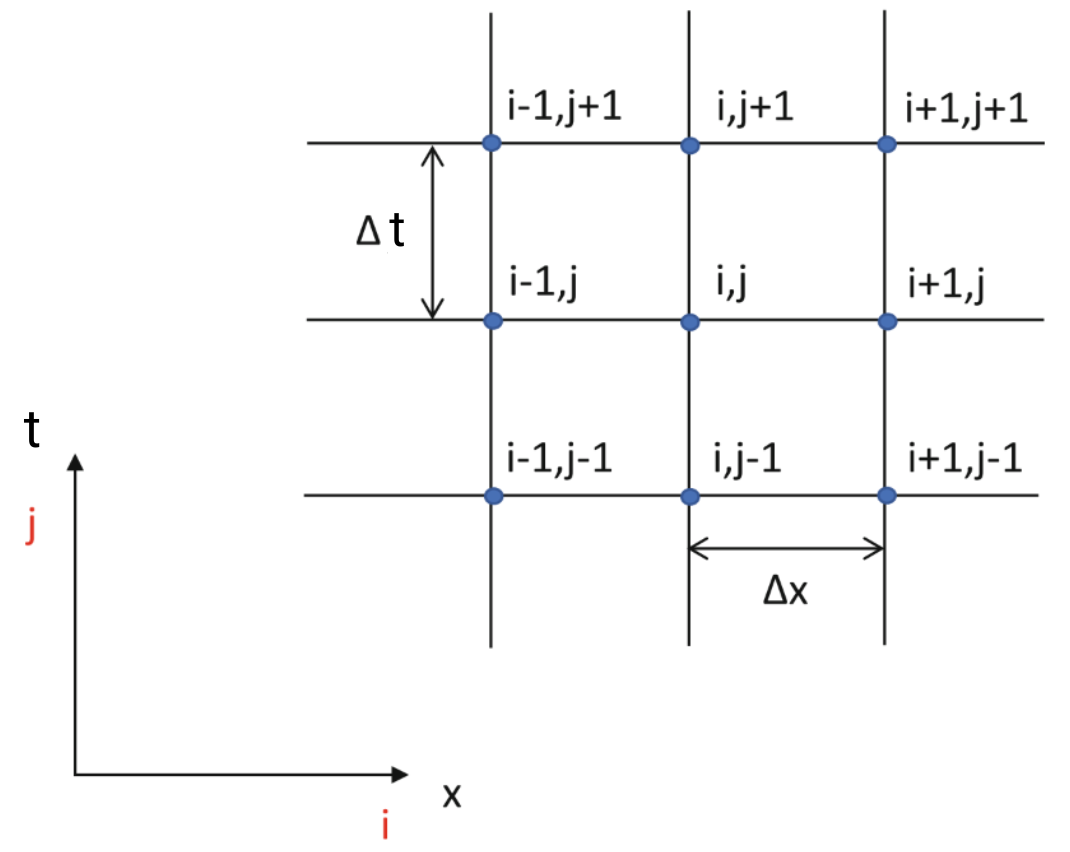
\includegraphics[width=0.48\textwidth]{figuras/grid.png}
        \caption[Grade para visualização do método das diferenças finitas]{Grade para visualização do método das diferenças finitas (adaptado de Lona, 2018).}
    \label{fig:grid}
\end{figure}

Portanto, discretizando as derivadas parciais, temos:

\begin{equation}
    \left( \frac{\partial C}{\partial t} \right)_{i,j} = \frac{C_{i,j+1} - C_{i,j}}{\Delta t}
\end{equation}

\begin{equation}
    \left( \frac{\partial^2 C}{\partial x^2} \right)_{i,j} = \frac{C_{i-1,j} - 2C_{i,j} + C_{i+1,j}}{(\Delta x)^2}
\end{equation}

Substituindo na equação original:

\begin{equation}
    \frac{C_{i,j+1} - C_{i,j}}{\Delta t} = D \frac{C_{i+1,j} - 2C_{i,j} + C_{i-1,j}}{(\Delta x)^2}
\end{equation}

Rearranjando para resolver $C_i^{j+1}$:

\begin{equation}
    C_i^{j+1} = C_i^j + \frac{D \Delta t}{\Delta x^2} (C_{i+1}^j - 2C_i^j + C_{i-1}^j)
\end{equation}

O método de diferenças finitas é amplamente utilizado para problemas de difusão e demais situações de estado transiente, devido à facilidade de implementação. Porém, trata-se de um método condicionalmente estável, ou seja, sua estabilidade está sujeita à chamada condição de \Sigla{Courant–Friedrich–Lecy}{CFL}, dada por:

\begin{equation}
    k \frac{\Delta t}{\Delta x^2} \leq \frac{1}{2}
\end{equation}

\noindent onde $k$ é um parâmetro característico do problema, que aqui corresponde ao coeficiente de difusão (Chicone, 2017). Nessa condição, o passo temporal ($\Delta t$) depende do menor comprimento da célula no domínio computacional, tornando-a muito restritiva para resolver problemas com materiais finos (Chung et. al, 2003). 

Devido à espessura das matrizes poliméricas tanto do adesivo transdérmico quanto do anel vaginal serem muito pequenas, foi necessário um número extremamente alto de pontos temporais para satisfazer a condição CFL. Isso, somado aos altos valores de tempo total da simulação, resultou em consumo excessivo de memória e longos tempos de execução, tornando inviável a utilização do método das diferenças finitas.

\subsubsection{Método de Crank-Nicolson}

Crank (1975) propõe o uso do método de Crank-Nicolson como alternativa para o método das diferenças finitas em problemas de difusão. Enquanto o método de diferenças finitas padrão utiliza o estado da variável em um instante de tempo específico, o método de Crank-Nicolson faz uma média entre o instante atual e o próximo, combinando informações dos estados em $j$ e $j+1$, aplicando diferenças finitas tanto no tempo quanto no espaço. A aproximação da derivada espacial passa a ser dada por:

\begin{equation}
\frac{C_i^{j+1} - C_i^j}{\Delta t} = D \frac{C_{i+1}^{j+1} - 2C_i^{j+1} + C_{i-1}^{j+1} + C_{i+1}^j - 2C_i^j + C_{i-1}^j}{2 \Delta x^2}
\end{equation}

\noindent onde:
\begin{itemize}
    \item \( C_i^j \) representa a concentração no ponto \( i \) e no instante \( j \),
    \item \( \Delta t \) é o intervalo de tempo,
    \item \( \Delta x \) é o passo espacial.
\end{itemize}

A equação acima pode ser reorganizada para obter a forma explícita da concentração em $j+1$:

\begin{equation}
- \frac{\alpha}{2} C_{i-1}^{j+1} + (1 + \alpha) C_i^{j+1} - \frac{\alpha}{2} C_{i+1}^{j+1} = \frac{\alpha}{2} C_{i-1}^j + (1 - \alpha) C_i^j + \frac{\alpha}{2} C_{i+1}^j
\end{equation}

\noindent onde \( \alpha = \frac{D \Delta t}{\Delta x^2} \).

Esta equação resulta em um sistema tridiagonal que pode ser resolvido para cada instante \( j+1 \). Em termos matriciais, pode-se representar o sistema linear para os valores de \( C_i^{j+1} \) da seguinte forma:

\[
\begin{pmatrix}
1 + \alpha & -\frac{\alpha}{2} & 0 & \cdots & 0 \\
-\frac{\alpha}{2} & 1 + \alpha & -\frac{\alpha}{2} & \cdots & 0 \\
0 & -\frac{\alpha}{2} & 1 + \alpha & \cdots & 0 \\
\vdots & \vdots & \vdots & \ddots & \vdots \\
0 & 0 & 0 & -\frac{\alpha}{2} & 1 + \alpha \\
\end{pmatrix}
\begin{pmatrix}
C_1^{j+1} \\
C_2^{j+1} \\
C_3^{j+1} \\
\vdots \\
C_n^{j+1}
\end{pmatrix}
=
\begin{pmatrix}
b_1 \\
b_2 \\
b_3 \\
\vdots \\
b_n
\end{pmatrix}
\]

\noindent onde, para cada ponto:

\[
b_i = \frac{\alpha}{2} C_{i-1}^j + (1 - \alpha) C_i^j + \frac{\alpha}{2} C_{i+1}^j.
\]

Esse tipo de método, em que as soluções de um conjunto de equações simultâneas são obtidas para cada passo temporal, é chamado método implícito. Apesar de envolver mais trabalho para calcular cada ponto, o método de Crank-Nicolson garante estabilidade para todo valor de $\alpha$, sem precisar satisfazer a condição CFL. Isso permite usar passos temporais maiores, conforme necessário (Crank, 1975). Assim, foi possível obter uma modelagem melhor para o adesivo e o anel, exigindo menos recursos computacionais e otimizando o tempo de execução. 

Finalmente, foram adicionadas verificações para garantir que a quantidade de EE liberada em um único dia não ultrapassasse os valores da literatura, sendo 20 \textmu para o adesivo e  15 \textmu para o anel (Barnhart et. al., 2005; Heuvel et al. 2005), e que a quantidade total liberada não ultrapassasse a quantidade de fármaco disponível na matriz. Dessa forma, o modelo se aproxima mais das restrições físicas conhecidas.

Os modelos foram implementados em Python, utilizando o ambiente do Google Colab. Foram plotados gráficos para a concentração ao longo de cada uma das matrizes, em diferentes períodos de tempo. Os códigos completos para esses modelos encontram-se no Apêndice A, nas seções A.1 e A.2.

\subsection{Contraceptivo oral combinado}

A liberação de etinilestradiol a partir da pílula anticoncepcional (COC) é representada pela \Sigla{equação diferencial ordinária}{EDO}:

\begin{equation}
    \frac{dC}{dt} = k_d (C_s - C)
\end{equation}

\noindent sendo que a concentração inicial é conhecida ($C = 0$). 

Para resolvê-la, optou-se por um método numérico que simula a expansão da EDO em série de Taylor, utilizada na solução analítica, sem a necessidade de calcular derivadas de ordem superior. Trata-se do método de Runge-Kutta de quarta ordem (RK4), que é altamente preciso, computacionalmente eficiente e de implementação relativamente simples. A expressão geral para esse método foi obtida a partir de Lona (2018), e está descrita a seguir.

\begin{equation}
    y_{i+1} = y_i + \frac{h}{6} (K_1 + 2K_2 + 2K_3 + K_4) 
\end{equation}

\noindent onde $h$ é o passo temporal e $K_1$, $K_2$, $K_3$ e $K_4$ são as primeiras quatro derivadas:

\begin{equation}
\begin{aligned}
    K_1 &= f(x_i, y_i) \\
    K_2 &= f(x_i + 0.5h, \, y_i + 0.5h K_1) \\
    K_3 &= f(x_i + 0.5h, \, y_i + 0.5h K_2) \\
    K_4 &= f(x_i + h, \, y_i + h K_3)
\end{aligned}
\end{equation}

Para refinar os resultados de acordo com a realidade física, foi adicionada uma restrição para que a concentração liberada não ultrapassasse a quantidade de princípio ativo disponível em uma pílula. 

O modelo também foi implementado em Python, com o objetivo de obter um gráfico da concentração de etinilestradiol no fluido gastrointestinal ao longo do tempo. O código encontra-se no Apêndice A, na seção A.3.

\subsection{Taxa de liberação}

Durante o desenvolvimento do modelo, definiu-se como foco o estudo da liberação do etinilestradiol a partir de cada uma das matrizes. Portanto, a fim de calcular a concentração liberada ao longo do tempo, não foram considerados quaisquer processos metabólicos que pudessem influenciar nesse valor, como a distribuição, a eliminação e a absorção do fármaco no corpo humano.

 A taxa de liberação é calculada tomando a diferença entre as concentrações em intervalos consecutivos de tempo. Para o adesivo transdérmico e o anel vaginal, foi utilizada, para cada ponto temporal, a média da concentração ao longo de todos os pontos espaciais naquele instante. Com isso, para todos os modelos, foi seguida a expressão:

\begin{equation}
    R(t) = \Delta C = C_t - C_{t-1}
\end{equation}

\noindent onde $R$ é a taxa de liberação em um instante $t$.

Foram plotados os gráficos de liberação para cada matriz separadamente utilizando o intervalo de aplicação de cada uma. Em seguida, foi plotado um único gráfico para todas, utilizando o maior intervalo de tempo (21 dias) e considerando reposições para a pílula e o adesivo. O código completo encontra-se na seção A.4 do Apêndice A.